%!TEX root = ../../main.tex

\section{Vandpumpe}
Til styring af dosering fra karret, anvendes en 12V inline pumpe  med tilhørende MOSFET-styringskreds. 
Vandpumpen virker ved at der påtrykkes en DC-middelspænding i form af et PWM-signal, herved kan styrken reguleres ved at justere dutycycle på PWM-signalet.
Den implementerede styringskreds ses på figur \ref{screenshot:Styringskreds} på side \pageref{screenshot:Styringskreds}, her forklares kredsløbet yderligere.
I databladet er opgivet at pumpen benytter 12V, og trækker 3A, dette giver en beregnet afsat effekt på 36W, se beregning herunder:

\begin{figure}[!h]
    \begin{align*}
        I &= 3 A \\ 
        V &= 12 V \\
        P &= I*V \\ 
        &= 36W
    \end{align*}
\label{eq:PumpeA}
\caption{Beregning af effekt i vandpumpen}
\end{figure}

Derudover er den interne modstand beregnet til:

\begin{figure}[!h]
	\begin{align*}
   		V &= 12 V \\ 
        I &= 3 A \\
        R &= \frac{V}{I} \\ 
        &= 4 \Omega
  	\end{align*}
\label{eq:pumpeOhm}
\caption{Beregning af indre modstand}
\end{figure}

Styringskredsen skal på baggrund af disse data designes til at håndtere en strøm på 3A, og en spænding på 12V. 


\newpage
\subsection{MOSFET-styringskreds}
Til kontrolkredsen er valgt at benytte en N-channel IRLZ44Z-MOSFET transistor i common-source-konfiguration. Denne type transistor er logic-level kompatibel, og har spænding/strøm-grænseværdier der opfylder kravene ovenfor.  
Logic-level kompatible betyder at $ V_{GS(th)} < 5V $ og derved kan MOSFET'en, alene drives fra en MCU, her en PSoC.
$ V_{GS(th)} $ er den threshold-spænding hvor transistoren går ”on”.


Det ses af grafen på figur \ref{screenshot:GateToSourceVoltage} at MOSFET'en ved en $ V_{GS} = 5V $, (ved $T_J = 25)$ tillader en strøm på 100A, dette er mere end rigeligt til opgaven.

\begin{figure}[!h]
	\centering
	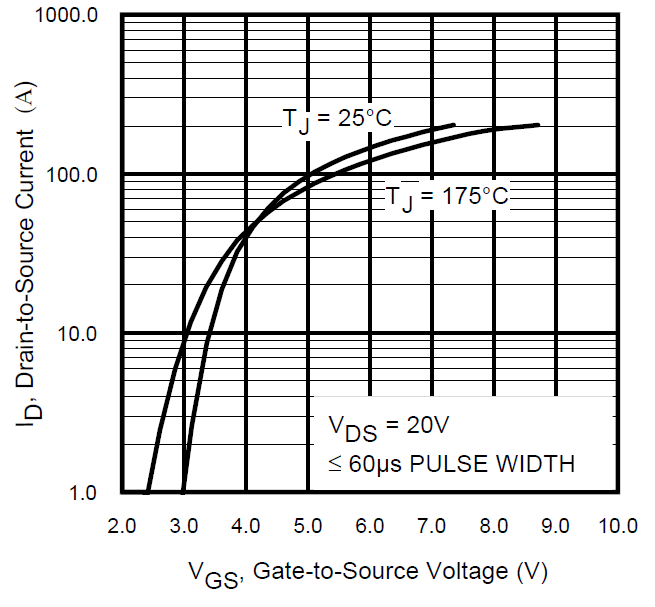
\includegraphics[scale=0.3]{../Hardware/Doseringspumpe/Screenshots/DatasheetGateToSourceVoltage}
	\caption{Datablad: Gate to Source voltage, fra databladets (Fig. 3, s.3)}
	\label{screenshot:GateToSourceVoltage}
\end{figure}

Ydermere kan det være interessant at se på hvor varm transistoren bliver under operation. Herved kan det udledes om der behøves ekstern køling eks. i form af en heat-sink.
Følgende værdier hentet fra databladet: 

\begin{figure}[!h]
	\begin{center}
		\begin{tabular}{ l l }
			 Drain to Source modstand:          & $R_{DS}=11 m\Omega$ \\ 
			 Strøm der trækkes af af relæet:    & $I = 3 A$ \\  
			 Junction-to-Ambient modstand:      & $R_{\theta JA}=62 C/W$ \\   
			 Max junction temp:                 & $Temp_{jun}=175 C$ \\
			 Ambient temp:                      & $Temp_{amb}=25 C$ \\
		\end{tabular}
	\end{center}
\caption{Værdier hentet fra datablad}
\end{figure}

Til beregningen benyttes formlen for afsat effekt: 

\begin{figure}[!h]
	\begin{align*}
		P_{afsat} &= R_{DS}*I^2 \\ 
		&= 99 mW
	\end{align*}
\caption{Afsat effekt i MOSFET}
\label{eq:afsatEffektMOSFET}
\end{figure}

Her ses det at under operation af pumpen afgiver transistoren 99 mW i varme. Ydermere noteres det, at den maksimale effekt der kan afsættes uden at der behøves heat-sink er 447.561mW. 

\begin{figure}[!h]
		\begin{align*}
			Temp_{max} &= \frac{(Temp_{jun}-Temp_{amb})}{R_{\theta JA}} \\ 
			&= 447.561 mW
		\end{align*}
\label{eq:maxMOSFETeffekt}
\caption{Max Temperatur uden heat-sink}
\end{figure}

Da der kun afsættes 99mW ved operation, er der ingen grund til at implementerer en heat-sink.

\subsubsection{Design af styringskredsløb}
På figur \ref{screenshot:Styringskreds}, ses MOSFET-styringskredsløb, PSoC'ens ”0” og ”1” er her simuleret ved en frekvensgenerator med tilpas lav frekvens.

\begin{figure}[!h]
	\centering
	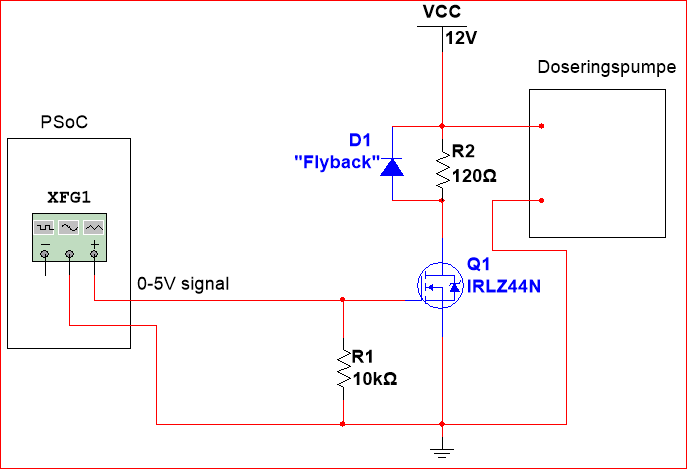
\includegraphics[height=7cm]{../Hardware/Doseringspumpe/Screenshots/DoseringspumpeStyringskredslob}
	\caption{Styringskredsløb til vandpumpe}
	\label{screenshot:Styringskreds}
\end{figure}

\paragraph{MOSFET-transistoren} \hspace{0pt} \\
Transistoren implementeres i common-source-konfiguration, for at et positivt signal på GATE til ”åbner” transistoren, og da den er en logic level model, stammer signalet direkte fra PSoC'en. 

\paragraph{Ground-modstanden} \hspace{0pt} \\
Der implementeres en modstand $R_1$ fra Gate til GND for at transistoren forbliver lukket (Gate trækkes til GND) hvis indgangssignalet til Gate afbrydes, dermed undgås det at GATE-signalet ”flyver” og transistoren potentielt kan stå og switche on/off hvis GATE afbrydes. $R_1$ implementeres med en $10k\Omega$s modstand, og virker som en standard ”pull down” resistor.

\paragraph{Flyback-diode} \hspace{0pt} \\
Derudover implementeres der, som førnævnt en ”flyback” diode, for at give strømmen en løbebane når relæet afbrydes. På denne måde indgås den høje $V_peak$ som spolen eller ville inducere, når der lukkes af for strømmen ændres monumentalt. Typen af diode, vælges ud fra følgende parametre:


\begin{description}
 \item[•] Hvilken strøm vil løbe i dioden
 \item[•] Hvilken Peak-spænding vil være over dioden
\end{description}

\subparagraph{Diode-strøm} \hspace{0pt} \\
Strømmen der vil løbe i dioden er givet fra databladet til  3A, derved skal den valgte diode kunne klare at lede max 3A, dette sker i forhold til spolens tidskonstant, $\tau$, hvor efter strømmen vil falde i løbet af $ 5 \tau$.

\subparagraph{Peak-spænding} \hspace{0pt} \\
Peak-spændingen fra spolen er realiseret i laboratoriet til 60V. \\ 

På baggrund af disse 2 værdier, vælges 1N4007, denne diode er, ifølge databladet i stand til at klare 1kVp, og 30A. Dette er tilstrækkeligt i denne situation.
